\documentclass[a4paper,12pt]{article}
\usepackage{amssymb}
\usepackage[portuguese]{babel}

\usepackage[utf8]{inputenc}
\usepackage[portuguese]{babel}
\usepackage[T1]{fontenc}
\usepackage{graphicx}
\usepackage[letterpaper,top=2cm,bottom=2cm,left=3cm,right=3cm,marginparwidth=1.75cm]{geometry}
\usepackage{float}

\title{Trabalho de Estrutura de Dados}
\author{ José Natan dos Santos \\Antonio Elivelton Moura Da Silva }
\date{Novembro 2022}

\begin{document}

\maketitle

\section{Introdução}
O intuito deste trabalho é implementar uma matriz esparsa usando liguagem C++. Este documento detalha os 4 arquivos utilizados para construir todo o programa, são eles: Node.h, SparseMatrix.h, SparseMatrix.cpp e main.cpp.
Para cada arquivo será descrito as suas principais partes e suas funções, assim como as ideias por trás da criação das mesmas.
Esse relátorio também apresenta uma seção com os códigos que podem ser utilizados ao executar o programa.
Um detalhe importante é que o relátorio possui diversas imagens sobre o código que está a ser descrito, e com as imagens é possivél ver os comentários feitos no código que poderão servir de complemento ao que está sendo descrito.
Um sengundo ponto importante é que algumas funções que possuem partes com implementação semelhante podem ter sido desenvolvidas de forma diferente mesmo tendo o mesmo objetivo, exemplo: utilizando uma função auxiliar para a resolução de uma etapa em uma dada função e em outra com a mesma etapa sendo utilizado uma implementação na própria função. 

\section{Comandos}
\begin{table}[H]
\begin{center}
\begin{tabular}{ |c|c|c| } 
    \hline
    Função & Comando & Variáveis \\ 
    \hline
    \hline
    Create & create l c & (número de linhas)(número de colunas) \\ 
    \hline
    Print & print id & (número da matriz) \\
    \hline
    Get & get id l c & (número da matriz)(número da linha)(número da coluna)\\
    \hline
    Remove & remove id l c & (número da matriz)(número da linha)(número da coluna)\\
    \hline
    Insert & insert id l c v & (matriz)(linha)(coluna)(valor a ser inserido)\\
    \hline 
    Mostrar todos & showAll & \\
    \hline
    Finalizar & end & \\
    \hline
    Somar & sum id1 id2 & (número das matrizes)\\
    \hline
    Multiplicar & multiply id1 id2 & (matriz A)(matriz B)\\
    \hline
    Ler Arquivo & read titulo.txt & (nome do arquivo)\\
    \hline
\end{tabular}
\caption{\label{tab:comandos} tabela de comandos}
\end{center}
\end{table}
\section{Classe Node}
\subsection{classe node private}
    
A classe node servirá para a criação dos nós da matriz esparsa, cada nó possui 5 valores:
Um valor para a identificar a linha, um valor para identificar a coluna, um valor do tipo double para a posição linha coluna e por fim dois ponteiros que apontarão para os próximos nós na mesma linha e coluna.
Essa classe também dará acesso ao seu conteudo para a classe SparseMatrix que será abordada mais adiante no relatório.

\begin{figure}[h]
\centering
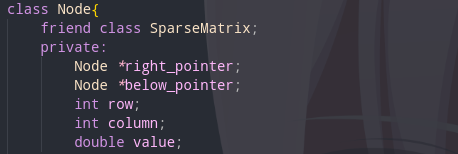
\includegraphics[width=1\textwidth]{Imagens/node/class-node-private.png}
\caption{\label{fig:nodeprivate} definição do private da classe node}
\end{figure}

\subsection{Classe node Public}
A classe node possui apenas um elemento na sua sessão public, que é o seu construtor. 
O construtor da classe node receberá valores referentes aos citados na sessão private e os atribuirá ao valores referidos.

\begin{figure}[h]
\centering
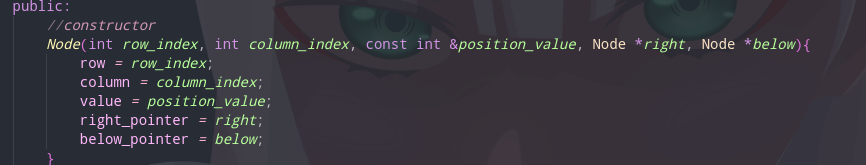
\includegraphics[width=1\textwidth]{Imagens/node/class-node-public.png}
\caption{\label{fig:nodepublic} definição do public da classe node}
\end{figure}

Sem muita complexidade ou dificuldades durante a construção do Node.h \\
após o seu construtor apenas encerramos o arquivo com o 'endif' e os nós estão prontos para serem utilizados.

\section{SparseMatrix.h}
\subsection{Definição das funções}

Este arquivo é também bem simples, possui apenas a definição das funções que serão implementadas no SparseMatrix.cpp, porém é válido comentar que os comentários com as descrições de cada função estão presentes aqui no SparseMatrix.h
A SparseMatrix é constituída de um nó cabeça e a quantidade de linhas e colunas como mostrado na figura \ref{fig:sparsematrixh1} abaixo: 

\begin{figure}[h]
\centering
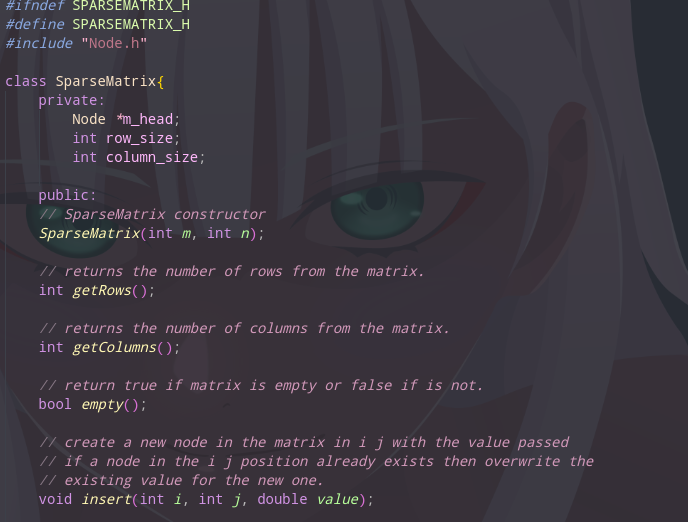
\includegraphics[width=1\textwidth]{Imagens/sparsematrixH/sparsematrixH-pt1.png}
\caption{\label{fig:sparsematrixh1} }
\end{figure}


Ao todo 10 funções foram definidas:

\texttt{ itemize }
\begin{itemize}
    \item SparseMatrix
    \item getRows
    \item getColumns
    \item empty
    \item insert
    \item get
    \item validatePosition
    \item print
    \item remove
    \item  \sim $SparseMatrix
\end {itemize}

\begin{figure}[H]
\centering
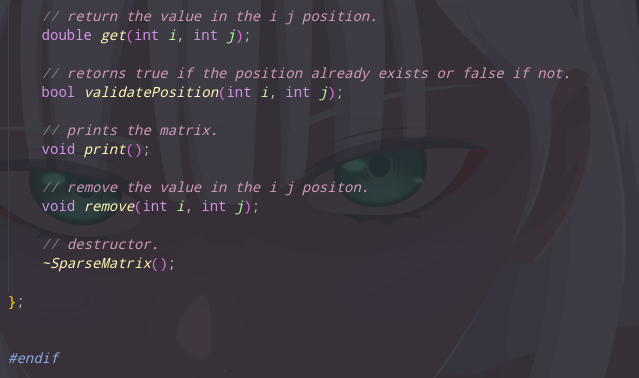
\includegraphics[width=1\textwidth]{Imagens/sparsematrixH/sparsematrixH-pt2.png}
\caption{\label{fig:sparsematrixh} definição das funções da sparsematrix}
\end{figure}

Nessas 10 funções estão inclusas as funções auxiliares, contrutor, destrutor e as funções principais. Todas elas serão descritas e explicadas na sessão SparseMatrix.cpp

\section{SparseMatrix.cpp}
Nessa sessão será aprofundaremos na implementação de cada função, explicando a lógica por de trás e apontando as dificuldades encontradas, assim como, uma análise da complexidade do pior caso das funções requisitas pelo PDF de instruções.

\subsection{Construtor}
O construtor da matriz esparsa, assim como o de uma matriz normal, receberá dois valores que definirão a quantidade de linhas e colunas da matriz.
Caso os valores passados para linha e coluna sejam abaixo de 0 uma exceção é lançada. 

\begin{figure}[H]
\centering
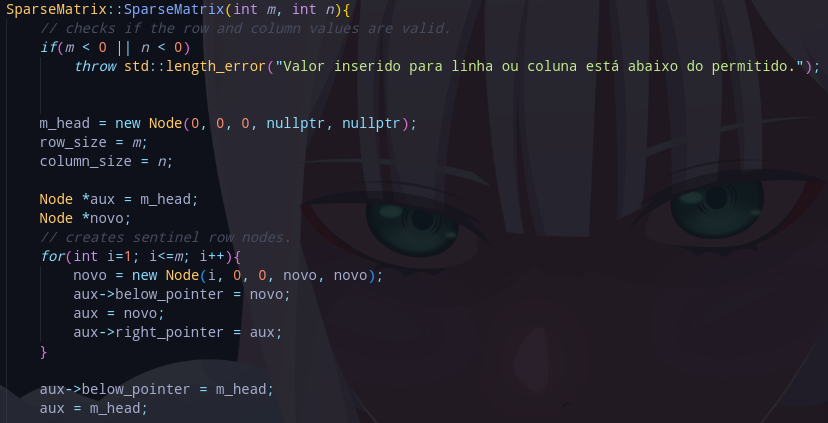
\includegraphics[width=1\textwidth]{Imagens/sparsematrixCPP/sparsematrix-construtor-pt1.png}
\caption{\label{fig:sparsematrix}}
\end{figure}

A ideia aqui é simples, a partir do nó sentinela(mHead) criar i nós para as linhas e j nós para as colunas, que servirão como nós cabeças para as suas respectivas posições.
Como as listas da matriz são circulares isso significa que cada novo nó apontará para si mesmo, com o ponteiro da direita ou o ponteiro para baixo, a depender de sua posição na matriz, e o ultimo nó da linha e coluna apontarão para o nó cabeça da matriz.

\begin{figure}[h]
\centering
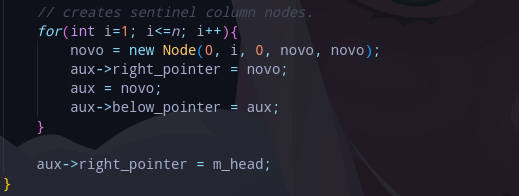
\includegraphics[width=1\textwidth]{Imagens/sparsematrixCPP/sparsematrix-construtor-pt2.png}
\caption{\label{fig:construtor}implementação do construtor}
\end{figure}

Dado ao uso de nós sentinelas em todas as linhas e colunas da matriz as suas posições válidas e que possuirão valores, começarão a partir da posição 1 e não da 0 como geralmente ocorre em outras estruturas de dados semelhantes a array.

\subsection{Empty}
Empty é uma função auxiliar que basicamente dirá se a matriz que a chamou está vazia ou não.
A lógica utilizada é simples, é criado um nó auxiliar que percorrerá todos os nós sentinelas referentes as linhas da matriz, e para cada linha é checado se existe algum nó existente naquela linha que não seja o próprio nó sentinela, ou seja, se existe de fato algum dado salvo na linha, essa checagem é feita olhando as colunas da mesma linha.
Se existir um valor na linha isso significa que a matriz não é vazia e a função retorna false, do contrário a função retorna true pois a matriz está vazia. 

\begin{figure}[h]
\centering
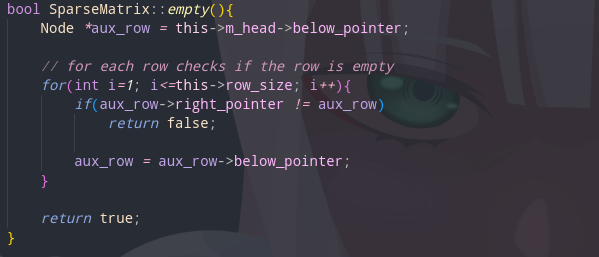
\includegraphics[width=1\textwidth]{Imagens/sparsematrixCPP/empty.png}
\caption{\label{fig:empty} função auxiliar empty}
\end{figure}


\subsection{Insert}
A função mais complexa da matriz esparsa, insert por sua vez tem uma missão muito simples, inserir um novo nó na posição i j da matriz e com o valor passado por parâmetro.
De início a função verifica se os valores de i e j passados por parâmetro estão dentro da margem da matriz, ou seja, se nenhum deles é maior que o número máximo de linhas e colunas da matriz, caso seja uma mensagem é imprimida na tela e a execução da função é cancelada.

\begin{figure}[H]
\centering
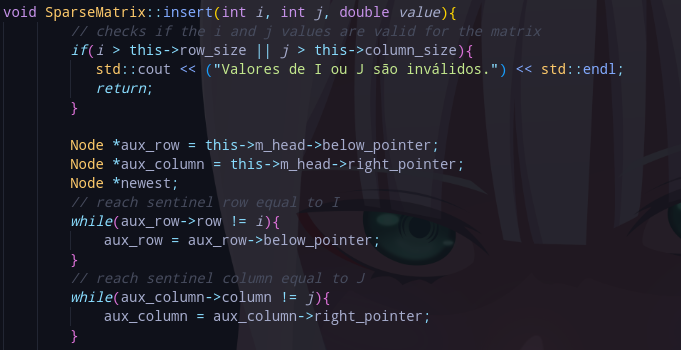
\includegraphics[width=1\textwidth]{Imagens/sparsematrixCPP/sparsematrix-insert-pt1.png}
\caption{\label{fig:insert} }
\end{figure}

Após a verificação é criado três nós, sendo dois deles auxiliares, um para as linhas da matriz e outro para as colunas, e o último será o nó a ser adicionado na matriz.
Os nós auxiliares irão percorrer a matriz até que estejam um na linha i e o outro na coluna j.\\
Em seguida é feita um checagem se matriz está vazia, utilizando a função auxiliar empty, caso a matriz esteja vazia significa que esse será o primeiro valor a ser inserido nela, então basta criar o novo nó e fazer ele apontar para os auxiliares e os auxiliares apontarem para ele.\\
Caso a matriz não esteja vazia as coisas ficam um pouco mais complicadas, por conta disso são feitos mais dois novos nós para facilitar a resolução do problema, esses nós servirão como auxiliares dos auxiliares já criados anteriormente, as coisas podem começar a ficar confusas mas é só questão de nomenclatura. Cada novo nó auxiliar receberá os nós que eles vão auxiliar, no caso temos o nó auxrow que é o nó auxiliar das linhas da matriz e ele possui agora um auxilar chamado auxr1 que é inicializado com auxrow, o mesmo vale para o auxiliar das colunas(auxcolumn).

\begin{figure}[H]
\centering
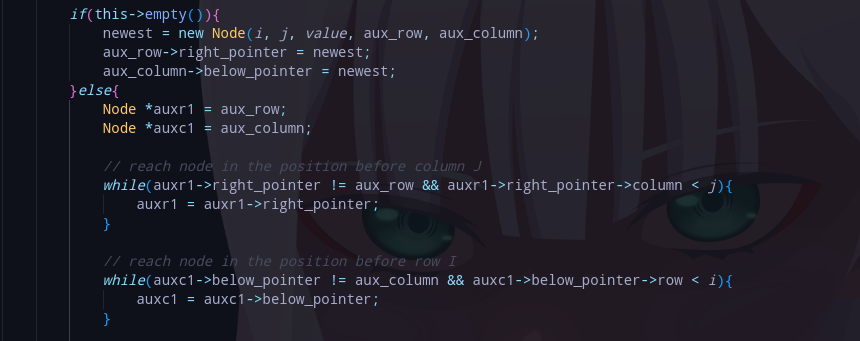
\includegraphics[width=1\textwidth]{Imagens/sparsematrixCPP/sparsematrix-insert-pt2.png}
\caption{\label{fig:insert}}
\end{figure}

Para quê esses novos auxiliares? Será necessário percorrer pelos nós dentro da matriz e ao mesmo tempo salvar os valores da linha sentinela i e coluna sentinela j, que são respectivamente o auxrow e auxcolumn. Os dois novos auxiliares irão percorrer a matriz, o novo auxiliar das linhas irá até o nó que antecede o nó na coluna j da mesma linha, equanto o novo auxiliar das colunas irá até a linha que antecede o nó na linha i da mesma coluna.\\
Depois de salvar a posição dos nós sentinelas i j, e dos nós que estão antes da posição que se deseja inserir um novo nó será necessário fazer o que? Isso mesmo criar mais nós auxiliares! Mas dessa vez serão chamados de temporários para evitar mais dores de cabeça, atente-se ao seguinte da mesma forma que o nó auxr1 é um nó auxiliar do auxrow, o novo nó temporario tempr é um nó auxiliar do auxr1, e o tempc do nó auxc1.

\begin{figure}[H]
\centering
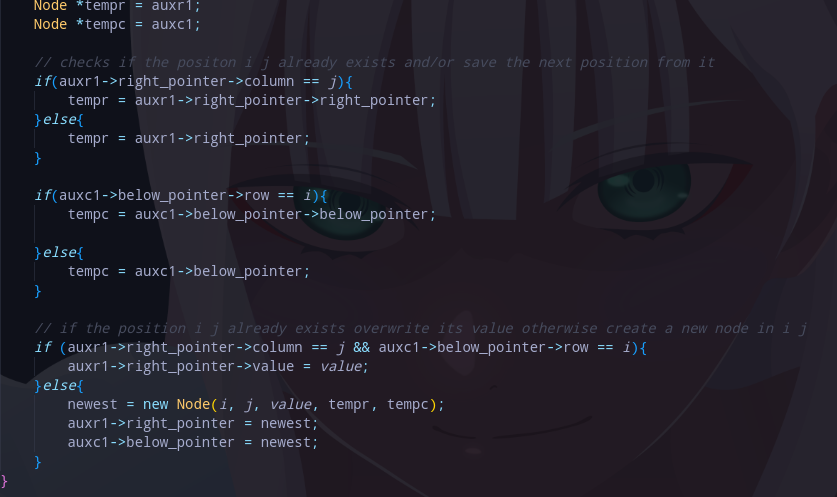
\includegraphics[width=1\textwidth]{Imagens/sparsematrixCPP/sparsematrix-insert-pt3.png}
\caption{\label{fig:insert} implementação do insert}
\end{figure}

 A função desses novos nós temporários é salvar o nó que se localiza após a posição i j, o motivo é que ao criar um novo nó será necessário fazer ele apontar para os nós seguintes da matriz, esses nós serão os auxiliares temporários, mas também será necessário fazer os nós que antecedem o novo nó apontar para ele, esses nós são os auxiliares dos auxiliares. Confuso? Sim, agora imagine pensar nisso.\\
 Por fim a função faz o que foi dito anteriormente percorre a matriz para salvar nos temporários os nós seguintes aos da posição i j, ela faz isso checando se após o nó na posição anterior a i j a coluna e linha dele é igual a i j, e aqui entra dois casos: Se os valores forem iguais significa que existe um nó naquela posição e o seu valor deve ser sobrescrevido, caso os valores não sejam iguais então não existe um nó na posição i j, é criado um novo nó e inserido nessa posição logo após isso a matriz é reajustada com os nós salvos no batalhão de auxiliares criados anteriormente.\\\\

 \textbf{ Análise de complexidade:}\\
A função insert no começo possui dois lados não aninhados que irão percorrer toda a matriz, continuando e considerando o pior caso a função executará mais dois laços que percorrerão toda a matriz novamente, inacreditavelmente a função insert no pior caso possui apenas laços não aninhados e não inclui a função auxiliar empty, porém a execução de seus laços se dá pelo valor de i j que não são necessariamente iguais, logo é correto afirmar que a complexidade do insert é O(i+j).

\subsection{Validate Position}
Validate Position é mais uma função auxiliar, foi criada por conta da necessidade de verificar se posições i j requeridas em certas funções existiam na matriz.
Como dito a função verifica a existência da posição i j, para isso ela recebe esses valores por parâmetro, e semelhante a função empty, será criado um nó auxiliar que percorrerá pelas linhas sentinelas da matriz até chegar na linha i.
Após concluir a primeira parte basta checar se na linha i existe um nó com o valor da coluna igual a j, caso ele exista então a função retorna true, se não ela retorna false.

\begin{figure}[H]
\centering
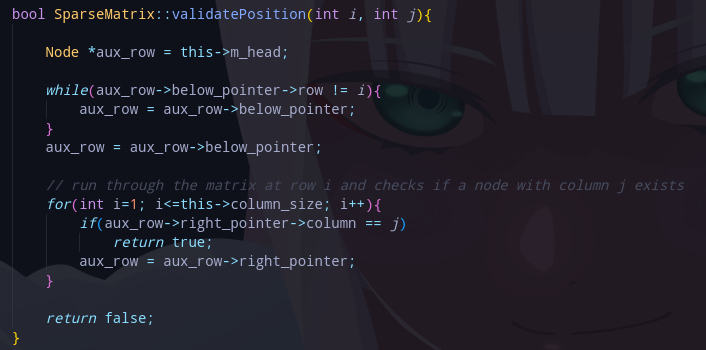
\includegraphics[width=1\textwidth]{Imagens/sparsematrixCPP/sparsematrix-validateposition.png}
\caption{\label{fig:validatepositon} função auxiliar validate position}
\end{figure}

\subsection{Get}
A função recebe dois valores por parâmetro que serão usados como linha e coluna de uma matriz, e ao fim o valor nessa posição deve ser retornado.\\
De inicio é feita uma verificação se a matriz é vazia e se os valores passados são de uma posição válida, caso a matriz não atenda a um desses requisitos é lançada uma exceção.\\
Em seguida é criado um auxiliar, assim como em outras funções ele irá percorrer a matriz até a linha i e o nó anterior ao nó da coluna j, vale informar que foi cogitada a criação de uma função auxiliar para fazer esses passos de pecorrer o vetor para a posição i e j, porém essa ideia se perdeu durante o desenvolvimento.\\
Por fim o valor na posição i j é retornada.

\begin{figure}[H]
    \centering
    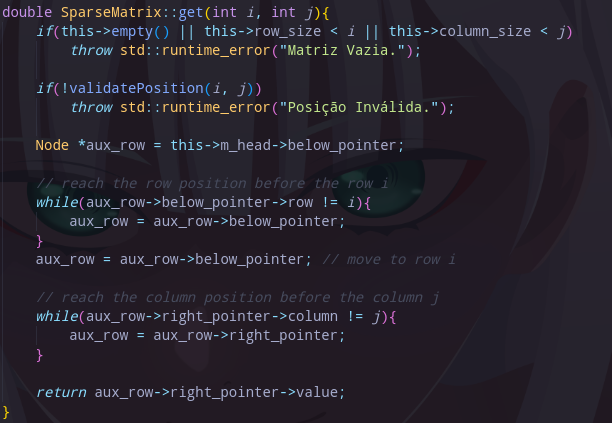
\includegraphics[width=1\textwidth]{Imagens/sparsematrixCPP/sparsematrix-get.png}
    \caption{\label{fig:get} função get}
\end{figure}

\textbf{Análise de complexidade:} \\
Existem dois laços na função get, o número de vezes que ambos os laços irão executar irá depender dos valores de i e j. Como o ponteiro já inicia no next do mhead o pior caso do primeiro laço seria quando o i fosse 1 e o auxiliar teria que percorrer todas as linhas inclusive voltar para o mhead para então encontrar a linha 1, o que seria equivalente a executar o laço rowSize(quantidade de linhas) vezes.
Para o segundo laço o pior caso fica ocorre quando j é igual ao número total de linhas, sendo assim sendo necessário percorrer por todas as colunas da matriz.\\
Como o número de vezes que os laços executam dependem do valor de entrada na função e os laços não são aninhdos a complexidade fica sendo O(n).

\subsection{Print}
O objetivo dessa função é imprimir na tela todos os valores da matriz que chamou a função, para uma melhor visualização essa impressão é feita no formato de tabela, com linhas e colunas simulando um desenho de uma matriz de fato. Existe uma restrição porém, a matriz esparsa permite que haja posições sem valores inseridos, o que formaria um espaço em branco na impressão, tendo em vista isso para cada posição i j na matriz que não possua um nó será imprimido um 0 no lugar.

\begin{figure}[h]
\centering
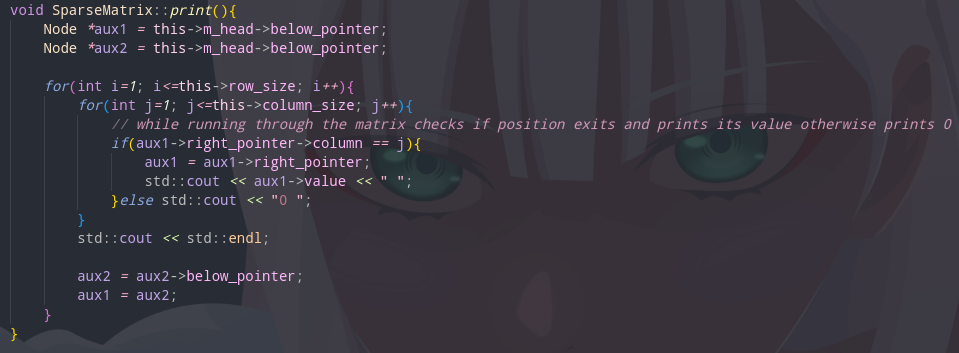
\includegraphics[width=1\textwidth]{Imagens/sparsematrixCPP/sparsematrix-print.png}
\caption{\label{fig:print} implementação da função print}
\end{figure}

A função começa criando dois nós auxiliares que percorrerão as linhas da matriz, o primeiro servirá para verificar se existe um nó na coluna j e na mesma linha que ele, caso exista então o seu valor é impresso do contrário um 0 é imprimido. O segundo nó terá o nó da linha salvo, passará a ter o nó sentinela da linha seguinte e o primeiro auxiliar receberá esse nó e repetirá o processo até finalizar todas as linhas da matriz.
Note-se que seria possível utilizar a função auxiliar Validate Position nessa função, porém dado a simplisidade da função print e como uma forma de mostrar uma resolução alternativa sem a ajuda de funções auxiliares, o print, foi feito dessa maneira.

\subsection{Remove}
Dado uma posição i j o remove irá deletar o nó na posição indicada.
Essa função é um bom exemplo de um bom uso de funções auxiliares, visto que antes de tudo é preciso fazer duas verificações na matriz, a primeira é saber se a matriz é vazia, pois caso seja não haverá nó a ser deletado, a segunda verificar se existe algum nó na posição i j para ser deletado. Para fazer essas verificações é utilizado as funções auxiliares empty e validate position, observe que mesmo tendo uma grande semelhança as duas possuem propósito e resultado diferentes, e o uso das duas evita de fazer uma função muito extensa e que faça muitas coisas.

\begin{figure}[h]
\centering
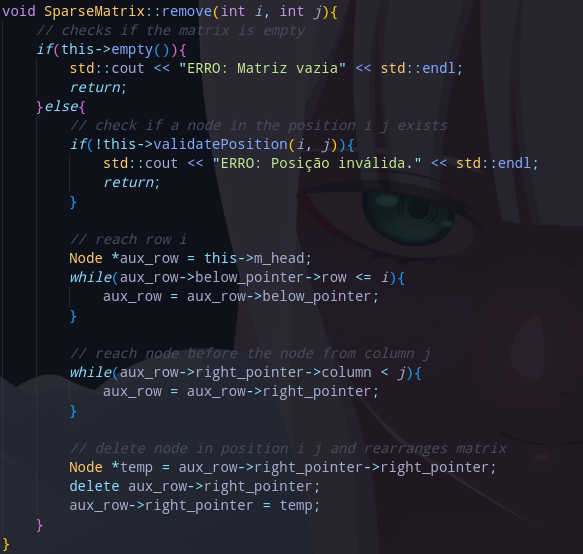
\includegraphics[width=1\textwidth]{Imagens/sparsematrixCPP/sparsematrix-remove.png}
\caption{\label{fig:remove} implementação da função remove}
\end{figure}

Após as verificações é criado um nó auxiliar, ele chegará na linha i e nessa mesma linha ele irá navegar até o nó que esteja antes do nó da coluna j, ou seja, o nó que o seu ponteiro da direita aponte para o nó i j, após isso o nó que é apontado pelo nó i j é salvo em uma variavel temporaria e finalmente o nó i j é deletado e a matriz é reajustada com o auxiliar apontando para o temporario.

\subsection{Destrutor}
Essa função é chamada na hora de deletar uma matriz da memória, para isso dentro da função um auxiliar percorre todos os nós sentinela e deleta um a um até que reste apenas o nó cabeça mhead, tendo apenas o mhead sobrando basta deletá-lo. 

\begin{figure}[h]
\centering
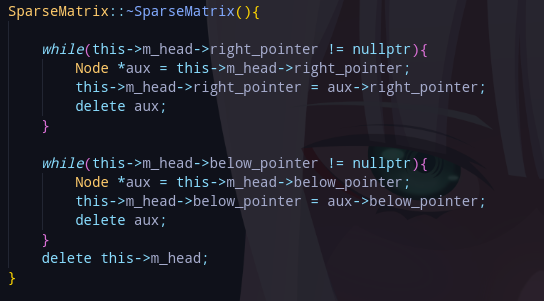
\includegraphics[width=1\textwidth]{Imagens/sparsematrixCPP/sparsematrix-destrutor.png}
\caption{\label{fig:remove} implementação do destrutor}
\end{figure}


\section{Main}
Nesse progama o arquivo main.cpp fica responsável por implementar as funções de leitura de arquivo e soma e multiplicação de matrizes, assim como os comandos utilizados para executar todo o programa e utilzar as funções.
Para poder rodar o programa por comandos de forma efetiva é criado um array que armazenará todas as matrizes criadas pelo usuário.\\
Todos os comandos estão especificados na tabela \ref{tab:comandos} na sessão 2.

\subsection{Implementação dos comandos}
Comando create utiliza o construtor para criar uma nova matriz e armazena ela no array de matrizes.\\
O comando print necessita de um id de uma matriz que na prática é o index em que se encontra a matriz desejada no array de matrizes.
\begin{figure}[H]
\centering
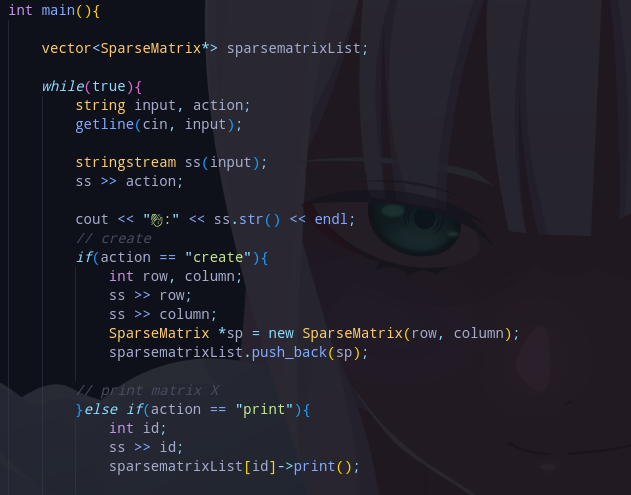
\includegraphics[width=1\textwidth]{Imagens/main/main-comandos-pt1.png}
\caption{\label{fig:createandprint} comandos create e print}
\end{figure}


\begin{figure}[H]
\centering
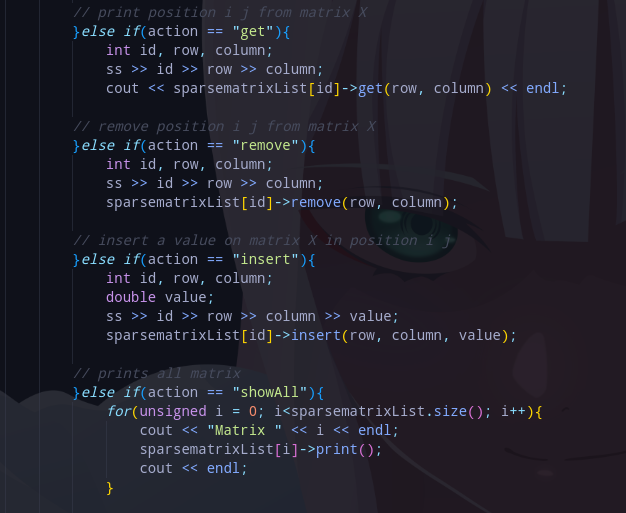
\includegraphics[width=1\textwidth]{Imagens/main/main-comandos-pt2.png}
\caption{\label{fig:gettoshowall} comandos get, insert, remove e showAll}
\end{figure}

\begin{figure}[H]
\centering
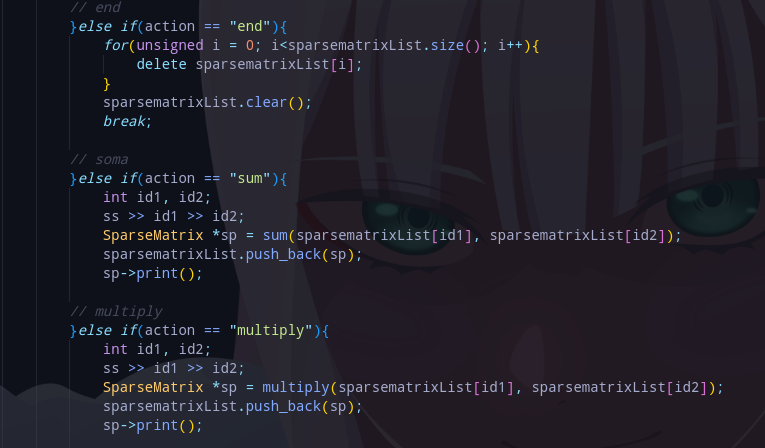
\includegraphics[width=1\textwidth]{Imagens/main/main-comandos-pt3.png}
\caption{\label{fig:endtomult} comandos end, sum e multiply}
\end{figure}

\begin{figure}[H]
\centering
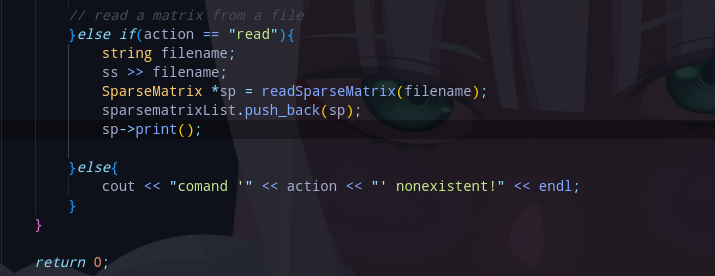
\includegraphics[width=1\textwidth]{Imagens/main/main-comandos-pt4.png}
\caption{\label{fig:readandelse} comando read e a exceção}
\end{figure}


\subsection{Soma}
O objetivo da função é pegar as duas matrizes que são passadas por parâmetro, somar elas e armazenar numa nova matriz que será inserida em um array na main.
Para começar a função verifica se as duas matrizes possuem o mesmo tamanho, caso sejam diferentes é lançada uma exceção.
Prosseguindo é criada uma matriz de mesmo tamanho que as duas matrizes que serão somadas, para cada posição i j é verificado atráves da função auxiliar validate position se existe um valor a ser somado nas duas matrizes na posição referenciada, caso haja o valor na posição i j na primeira matriz é somado com o valor da segunda matriz na mesma posição e armazenado na nova matriz. Caso apenas uma das duas matrize não possua um nó na posição i j a nova matriz recebe na mesma posição o valor da matriz que possue um nó em i j. 

\begin{figure}[H]
\centering
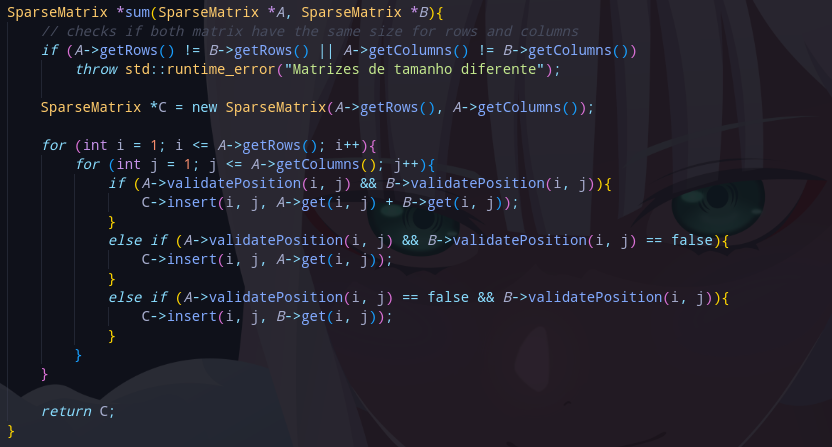
\includegraphics[width=1\textwidth]{Imagens/main/soma-matriz.png}
\caption{\label{fig:sum} função somar matrizes}
\end{figure}

\textbf{ Análise de complexidade:}\\
De cara é possível notar que a função utiliza laços aninhados e sabendo que sempre é necessário percorrer toda a matriz para efetuar a soma de todas as posições a função poderia ser definida com complexidade O(n²), porém existe a utilização de uma função auxiliar em todos os casos verificados pela função soma, a função validate position por si só possui uma complexidade de O(n), é possível enxergar essa complexidade na sessão que explica a validate position. Sabendo disso a função de soma sempre irá percorrer as duas matrizes sempre irá executar o validate position em ambas as matrizes, resultando em uma complexidade de O(n² + n) ou O(n²) + O(n), algo nesse sentido.

\subsection{Multiplicação}
A função multiply recebe duas matrizes por parâmetro e começa verificando se o número de colunas da primeira matriz é igual ao número de linhas da segunda, já que essa é uma condição para a realização de uma multiplicação entre matrizes. Uma exceção é lançada caso os valores sejam diferentes.

\begin{figure}[H]
\centering
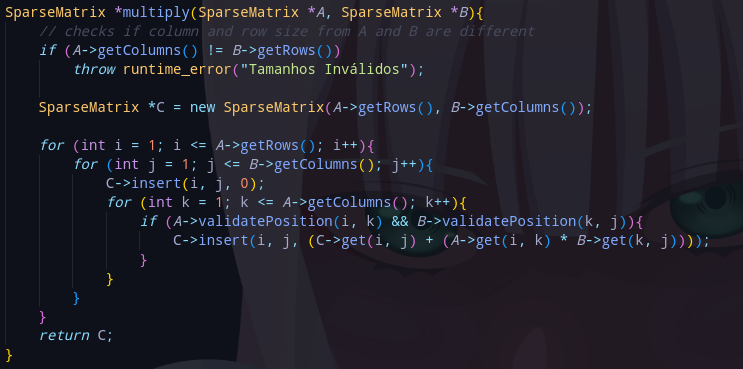
\includegraphics[width=1\textwidth]{Imagens/main/multiplicacao-matriz.png}
\caption{\label{fig:mult} função multiplicar matrizes}
\end{figure}

Após a verificação é criada uma nova matriz tendo o número de linhas da primeira e o número de colunas da segunda depois os passos padrões para a efetuação de uma multiplicação de matrizes são feitos, basicamente cada linha da primeira matriz é multiplicada pelas colunas da segunda matriz.


\subsection{Ler arquivo}
A função recebe o nome de um arquivo.txt, a partir desse arquivo é feita uma leitura específica nele. Para os dois primeiros valores lidos do arquivo é criada uma nova matriz que tenha o primeiro valor como o número de linhas e o segundo valor do arquivo como número de colunas.

\begin{figure}[H]
\centering
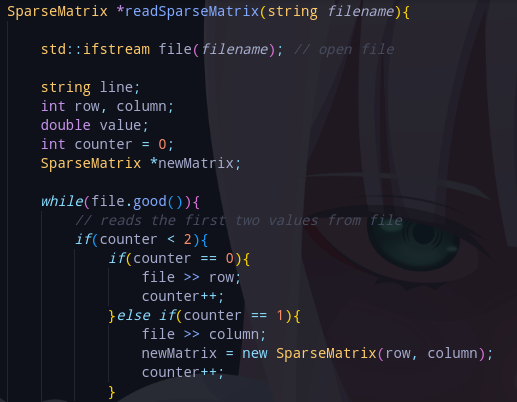
\includegraphics[width=1\textwidth]{Imagens/main/read-sparsematrix-pt1.png}
\caption{\label{fig:readt}}
\end{figure}

O restante do arquivo é lido e a cada três valores é inserido na nova matriz um nó com os ultimos dados lidos sendo eles a linha, coluna e valor do nó respectivamente. Após todo o arquivo ser lido a função fecha o arquivo e retorna a nova matriz, que será armazenada no array de matrizes.


\begin{figure}[H]
\centering
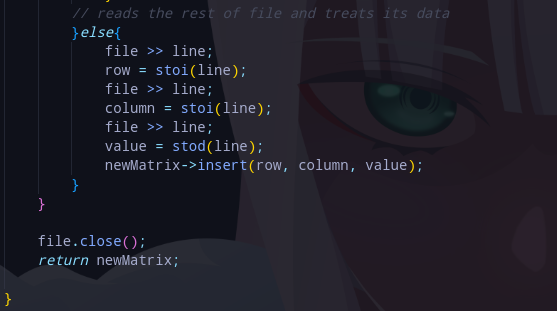
\includegraphics[width=1\textwidth]{Imagens/main/read-sparsematrix-pt2.png}
\caption{\label{fig:read} função de leitura de arquivo}

\end{figure}
 
 
 \section{Divição das Tarefas }
 
  O trabalho foi dividido em blocos, cada um ficou resposável por criar funções que iriam fazer o projeto funcionar, corretamente depois juntamos tudo para fazer pequenas alterações necessárias, a elaboração do relatorio foi feita em conjuto.

\section{Referências}

Monitor da disciplina.
\end{document}
